%%% lorem.tex --- 
%% 
%% Filename: lorem.tex
%% Description: 
%% Author: Ola Leifler
%% Maintainer: 
%% Created: Wed Nov 10 09:59:23 2010 (CET)
%% Version: $Id$
%% Version: 
%% Last-Updated: Wed Nov 10 09:59:47 2010 (CET)
%%           By: Ola Leifler
%%     Update #: 2
%% URL: 
%% Keywords: 
%% Compatibility: 
%% 
%%%%%%%%%%%%%%%%%%%%%%%%%%%%%%%%%%%%%%%%%%%%%%%%%%%%%%%%%%%%%%%%%%%%%%
%% 
%%% Commentary: 
%% 
%% 
%% 
%%%%%%%%%%%%%%%%%%%%%%%%%%%%%%%%%%%%%%%%%%%%%%%%%%%%%%%%%%%%%%%%%%%%%%
%% 
%%% Change log:
%% 
%% 
%% RCS $Log$
%%%%%%%%%%%%%%%%%%%%%%%%%%%%%%%%%%%%%%%%%%%%%%%%%%%%%%%%%%%%%%%%%%%%%%
%% 
%%% Code:

\chapter{Method}
\label{cha:method}

\section{Pre-processing}\label{pre-processing}
\label{sec:pre-processing}
The complete dataset that was delivered by Östgötatrafiken is over 300GB in size, comprising of over half a billion rows. The data contains, among other things, GPS coordinates and different types of events representing actions performed by a bus. 

Since this data was unstructured in many ways, there was a need to transform it into a format that supports querying. By streaming over and parsing the raw log files, a subset of the data could be entered into pandas data frames. Operations such as filtering and plotting the statistical distributions of the raw data provided an initial overview of the dataset. This would, in turn, facilitate the creation of a simple finite state machine, which could extract data covering a complete journey from a specific bus line. This "clean" data could then be used as input to train our models.

\subsection{Data structure}
The provided data consists of one file per day, with a total of 92 days between February and April in 2018. Each file has an approximate size of 5GB, with around 2.4M rows per file. Within these files are logs over the \textit{events}, which each bus sends throughout the day. The events represent different states of the bus, and there are over 20 different event-types. For this project, only four event-types were needed to successfully extract complete journeys that could be used as input for our models. These four events, and what we use them for, are listed below:\\
\begin{description}
\item[ObservedPositionEvent:] Is sent by buses with a frequency of 1Hz. Contains (among other things) the GPS data, speed, and direction (angle) of a given bus. These events make up the bulk of the input to our models.
\item[EnteredEvent:] Is triggered when the bus is within a certain distance to a bus station. These events are used to split a journey into segments.
\item[JourneyStartedEvent:] Is triggered when the bus is assigned a new journey. These events are used to determine which line a bus is currently serving.
\item[JourneyCompletedEvent:] Is triggered when the bus has completed a journey. These events are used as a flag to determine when a journey has ended.
\end{description}

For this project, two bus lines were selected: bus lines number three and number eleven. For both lines, only the journeys going in one direction were used. For line three, a subset of the segments from an intermediate bus stop until the last bus stop was selected. The reason for not using the complete journeys (i.e. from the first to the last bus stop) is because there was construction work being performed on some bus stops during this time. This created inconsistencies in the data with regards to the path buses drove. 

Line three was chosen because we were familiar with this line, and knew its irregularities during the time period. This line also had less noise in the GPS signal due to the absence of tall buildings along the route. Conversely, line eleven (seen in Figure \ref{fig:211_stations}) was chosen because it captures many problems that need to be taken into consideration within our predictions. These include GPS noise due to nearby tall buildings and more heterogeneous GPS data between journeys due to a higher density of red lights and more traffic congestion.

\begin{figure}[!b]
\begin{minipage}{.5\textwidth}
    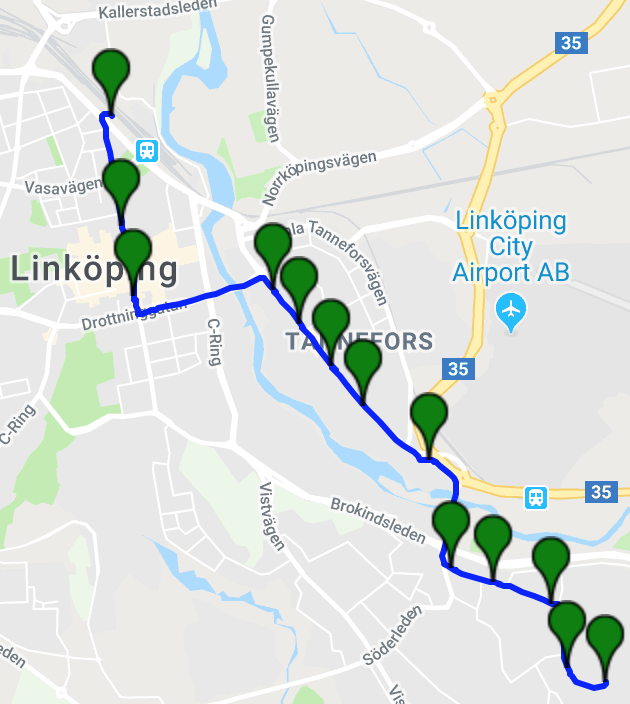
\includegraphics[scale=0.48,width=\textwidth]{211_stations}
    \caption{This figure shows a complete journey of the bus line eleven. The markers in green are events of type EnteredEvent. These events are triggered when the bus reaches within a certain distance of a station, and have been used to divide journeys into segments.}
    \label{fig:211_stations}
\end{minipage}
\hspace{5pt}
\begin{minipage}{.48\textwidth}
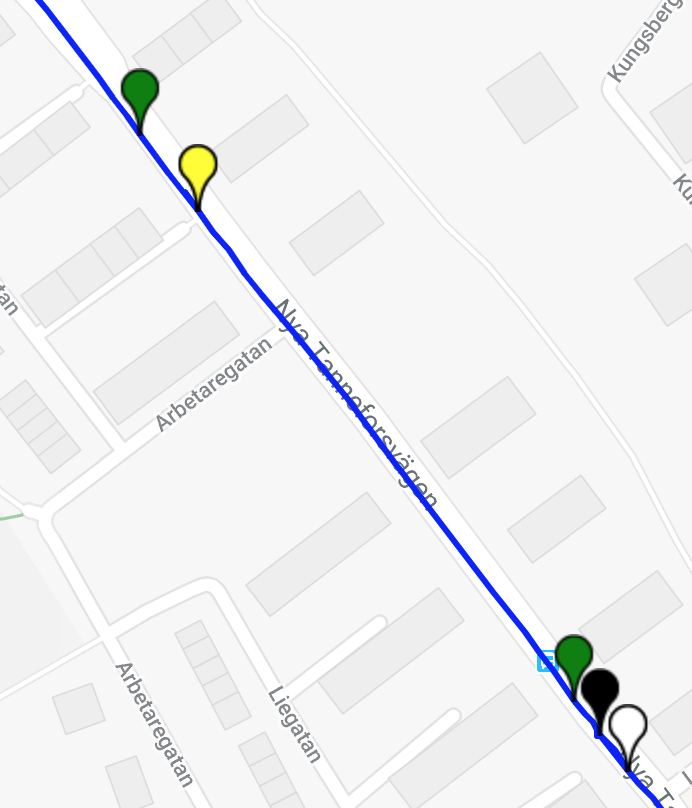
\includegraphics[scale=0.5,width=\textwidth]{entered}
\caption{In this figure, the bus passed the station in the upper left of the figure without stopping. Since the events for \textit{stopping} at a station doesn't get fired then (the black and white markers in the lower right of the figure), the EnteredEvent is used instead.}
\label{fig:entered}
\end{minipage}
\end{figure}


\subsection{Detecting Segments}
Bus journeys are split into several segments. The \textit{EnteredEvent} is used to detect when a bus is approaching a station and is also used to split the raw data into segments.  We first tried to use the \textit{StoppedEvent} for segment detection, but as seen in Figure \ref{fig:entered}, that event is not suitable. This is because this event "skips" some stations because there are no people trying to get on or off the bus.

The first segment of a journey starts when a \textit{JourneyStartedEvent} triggers. When all the journeys of interest have been collected from the raw data, the collection is investigated in order to find and remove severe anomalies (such as drivers taking a wrong turn). These faulty journeys are discarded since it is not feasible to create a model which takes such complexity into consideration, given the amount of training data available.

\section{Model evaluation}
To evaluate the performance of the models, we make four travel time predictions per segment in each journey. All predictions estimate the remaining travel time until the end of the segment (until the next bus stop). There is one prediction each being made once the bus has travelled 20\%, 40\%, 60\%, and 80\% of the total segment. All the models use an 80/20 split of the data into train/test sets, and use MAPE to evaluate.

\section{Baseline Method}
As a baseline model for segment time prediction, we calculate the median travel time for each part of the segments in the training data (in increasing 20\% intervals, as described above). Each median of the segment intervals is used to predict the remaining travel time of the corresponding segment interval in the test data.

\section{Artificial Neural Networks}

Artificial neural networks have shown to be useful when predicting travel times due to their ability to model nonlinear relationships between features \cite{brazilANN}\cite{malaysiaANN}. This section introduces some concepts and parameters that have been considered when creating artificial neural networks for this report followed by an explanation of how the models were created and evaluated.

\subsection{Activation Functions}
The purpose of the activation function is to compute the hidden layer values \cite{Goodfellow-et-al-2016}. Some popular activation functions are the sigmoid function:

\begin{equation} 
    f(x) = \frac{1}{1+e^{-x}} 
\end{equation}

the rectifier function:

\begin{equation} 
    f(x) = max\{0,x\}
\end{equation}

and \textit{tanh}:
\begin{equation} 
    f(x) =  \frac{e^x-1}{e^{x}+1} 
\end{equation}

All three have been considered for the models in this report but only the rectifier function and \textit{tanh} are used in the models. They have been chosen through parameter optimisation and some reasoning. For example, the output neuron of each model uses the rectifier function since the output should not be a negative value.

\subsection{Recurrent Neural Networks}
Recurrent neural networks (RNN) are a type of neural networks that can be used to make predictions based on a time-series \cite{RNN}. Instead of treating each data point independently like in a regular artificial neural network, an RNN handles sequences of data points which are continuous in time making it possible to take previously observed data points into account. They have been used to predict bus travel times, and the best results were achieved using Long short-term memory (LSTM) nodes \cite{RNNBusPredictions}. One of the models that are implemented in this report is an RNN. 

\subsection{Kalman Filters}
Kalman filtering is an iterative algorithm used to increase measurement accuracy by considering multiple consecutive data points observed over time. It can be used in real time as new measurements are made. Kalman filtering has been shown to be useful when predicting travel times \cite{kalmanPrediction}. It has also been used together with artificial neural networks with promising results \cite{kalmanANN}.

\subsection{Implementation}
A number of different neural network models were implemented and tested. The models were created using \textit{Keras}\footnote{https://keras.io/} on top of \textit{Tensorflow}\footnote{https://www.tensorflow.org/}. The created models were both based on suggestions by papers and new ideas because of the richness of features in the Östgötatrafiken dataset. All models will not be mentioned in this report, only the most significant ones. Featured models will be referenced by their notebook name. The implementation follows a three-step process which will be described step-wise below. Each step refers to a different notebook.

\subsection{Step 1 - Additional Pre-processing}
Some additional pre-processing was required to train the ANN models. Most importantly the data needs to be labelled with the correct labels used to train the models. Datasets acquired from the pre-processing described in section \ref{pre-processing} were complemented with the columns

\begin{itemize}
    \item The time it takes to travel the entire current segment (seconds) - Used in Model 1
    \item The time left until next bus stop (seconds) - Used in Models 2,3,4
    \item The time from the start of the journey to the start of the current segment (seconds) - Used in all models
    \item History with the three latest GPS coordinates and speed entries.
\end{itemize}

\noindent The first two columns that are added are used as true labels in the respective models. The third one is a feature which captures conditions earlier in the journey. The last column is used to let the network capture traffic conditions.

\subsection{Step 2 - Model Creation}
Each model was implemented separately. Each notebook containing a model takes the data from the previous step and outputs a new data frame with 

\begin{itemize}
    \item segment number
    \item journey number
    \item speed
    \item prediction
    \item label.
\end{itemize}

Where prediction is calculated once per input entry, this was made with the intent of creating easily comparable models.


\subsection{Model 1}
This model was created based on the structure described by Fan and Gurmu \cite{brazilANN}. The model predicts the time it takes to travel the current segment. It is assumed that the time is known when the bus left the latest station. Then, the time left to the next station is calculated by subtracting the time that has passed from the current station from the segment travel time prediction.

\subsection{Model 2}\label{M2}
With this model, the idea was to let the model itself predict the time left to the next segment, in contrast to Model 1. Also, more features are added.

\subsection{Model 3}\label{M3}
This model is very similar to Model 2 with the addition of history from the three latest samples of position and speed data.

\subsection{Model 4}
This model takes a different approach than model 3 to take the history into account. It is a recurrent neural network taking a sequence of 20 consecutive data points as input. It is predicting the time left to the next bus stop like model 2 and 3. 

\subsection{Stop-compressed models}
Models M1 through M4 were also evaluated with data that was stop-compressed (as described in section \ref{sec:stop-compression}) before calculating \textit{MAE} and \textit{MAPE}. 

\subsection{Layers}
Table \ref{tbl:nn-layers} presents the layer types and activation functions that were used during model creation. Models M1-M3 are regular ANNs, and were trained using the same parameters. This with the intent of letting the different features affect performance.

\begin{table}[H]
  \centering
  \caption{ANN layers used for different models. FC = \textit{Fully Connected}.}
  \label{tbl:nn-layers}
  \begin{tabular}{l|l|l|l|l}
        & \multicolumn{4}{c}{Models}                                                                                           \\ \cline{2-5} 
        & \multicolumn{2}{c|}{M1, M2, M3}                           & \multicolumn{2}{c}{M4}                                   \\ \hline
  Layer & Type                     & Activation                     & Type                     & Activation                     \\ \hline
  1     & FC, 2 * \#features nodes & RelU                           & LSTM, 128 nodes          & Tanh                        \\
  2     & FC, 1 * \#features nodes & Tanh                           & LSTM, 128 nodes          & Tanh                        \\
  3     & FC, 1 * \#features nodes & \textit{None} & LSTM, 128 nodes          & Tanh                        \\
  4     & output, 1 node           & RelU                           & FC, 32 nodes & RelU                           \\
  5     &                          &                                & output, 1 node           & RelU
  \end{tabular}
  \end{table}

\subsection{Features}
Table \ref{tbl:nn-features} describe the features used is the different models. Note that model M4 is does not have the two last features (7 and 8), instead it captures this with a sequence of 20 data points with all other features.

\begin{table}
  \caption{Features used in the different ANN models}
  \label{tbl:nn-features}
\begin{adjustbox}{center}
  \begin{tabular}{l|llll}
          & \multicolumn{4}{c}{Model}                                                                                                                                                                                                                                                                                                                                                                                                                                                                                                                \\ \hline
  Feature & \multicolumn{1}{l|}{M1}                                                                                                               & \multicolumn{1}{l|}{M2}                                                                                                               & \multicolumn{1}{l|}{M3}                                                                                                               & M4                                                                                                               \\ \hline
  1       & \multicolumn{1}{l|}{\begin{tabular}[c]{@{}l@{}}Segment number\\ (1-hot-encoded)\end{tabular}}                                         & \multicolumn{1}{l|}{\begin{tabular}[c]{@{}l@{}}Segment number\\ (1-hot-encoded)\end{tabular}}                                         & \multicolumn{1}{l|}{\begin{tabular}[c]{@{}l@{}}Segment number\\ (1-hot-encoded)\end{tabular}}                                         & \begin{tabular}[c]{@{}l@{}}Segment number\\ (1-hot-encoded)\end{tabular}                                         \\ \hline
  2       & \multicolumn{1}{l|}{Time of day (hour)}                                                                                               & \multicolumn{1}{l|}{Time of day (hour)}                                                                                               & \multicolumn{1}{l|}{Time of day (hour)}                                                                                               & Time of day (hour)                                                                                               \\ \hline
  3       & \multicolumn{1}{l|}{\begin{tabular}[c]{@{}l@{}}Time travelled until \\ the start of the current\\ segment, (normalised)\end{tabular}} & \multicolumn{1}{l|}{\begin{tabular}[c]{@{}l@{}}Time travelled until \\ the start of the current\\ segment, (normalised)\end{tabular}} & \multicolumn{1}{l|}{\begin{tabular}[c]{@{}l@{}}Time travelled until \\ the start of the current\\ segment, (normalised)\end{tabular}} & \begin{tabular}[c]{@{}l@{}}Time travelled until \\ the start of the current\\ segment, (normalised)\end{tabular} \\ \hline
  4       & \multicolumn{1}{l|}{}                                                                                                                 & \multicolumn{1}{l|}{\begin{tabular}[c]{@{}l@{}}Bus direction \\ (degrees, cyclical)\end{tabular}}                                     & \multicolumn{1}{l|}{\begin{tabular}[c]{@{}l@{}}Bus direction \\ (degrees, cyclical)\end{tabular}}                                     & \begin{tabular}[c]{@{}l@{}}Bus direction \\ (degrees, cyclical)\end{tabular}                                     \\ \hline
  5       & \multicolumn{1}{l|}{}                                                                                                                 & \multicolumn{1}{l|}{\begin{tabular}[c]{@{}l@{}}Bus speed \\ (m/s, normalized)\end{tabular}}                                           & \multicolumn{1}{l|}{\begin{tabular}[c]{@{}l@{}}Bus speed \\ (m/s, normalized)\end{tabular}}                                           & \begin{tabular}[c]{@{}l@{}}Bus speed \\ (m/s, normalized)\end{tabular}                                           \\ \hline
  6       & \multicolumn{1}{l|}{}                                                                                                                 & \multicolumn{1}{l|}{\begin{tabular}[c]{@{}l@{}}Bus GPS position \\ (normalized)\end{tabular}}                                         & \multicolumn{1}{l|}{\begin{tabular}[c]{@{}l@{}}Bus GPS position \\ (normalized)\end{tabular}}                                         & \begin{tabular}[c]{@{}l@{}}Bus GPS position \\ (normalized)\end{tabular}                                         \\ \hline
  7       & \multicolumn{1}{l|}{}                                                                                                                 & \multicolumn{1}{l|}{}                                                                                                                 & \multicolumn{1}{l|}{\begin{tabular}[c]{@{}l@{}}Bus GPS position \\ (history, 3 time steps)\end{tabular}}                              &                                                                                                                  \\ \hline
  8       & \multicolumn{1}{l|}{}                                                                                                                 & \multicolumn{1}{l|}{}                                                                                                                 & \multicolumn{1}{l|}{\begin{tabular}[c]{@{}l@{}}Bus speed \\ (history, 3 time steps)\end{tabular}}                                     &                                                                                                                 
  \end{tabular}

\end{adjustbox}
\end{table}

\subsection{Step 3 - Evaluation}
\textit{Notebook: 3. Evaluation.ipynb}
\newline
As the last step, the models were compared with the \textit{Mean Absolute Error} and are presented one random journey at a time. The loss in the model was also compared with the data without the first segment, as this segment showed to include a lot of dwell time, heavily impacting the performance. Finally, as some papers have shown good results [ref], a Kalman Filter is applied on top of the predictions.

\section{Gaussian Processes regression for trajectory data}
This section presents how trajectory based GP regression is used to predict the arrival times. The core concept of the model is that each trajectory $X_t$ and corresponding arrival time vector $Y_t$ is considered a realisation of a Gaussian Process(GP) which models the function $Y_t = f^{(t)}(X_t)$. A Gaussian Process (\textit{GP}) generalises a multivariate normal distribution, and is a distribution over functions~\cite{Rasmussen-Williams-2006}, completely defined by its mean function $m(x)$ and covariance function $k(x, x')$. For any input vector $x$ to these functions the output $y$ is jointly Normally distributed according to
\begin{equation}
  \label{eq:gp}
  y = f(x) \sim \mathcal{N}(\mu(x), \Sigma(x))
\end{equation}
where
\begin{equation}
  \label{eq:gp-mean-function}
  \mu(x) = m(x) + K(x, \textbf{x})\textbf{V}^{-1}{(y-m(x))}^{T}
\end{equation}
\begin{equation}
  \label{eq:gp-covariance-function}
  \Sigma(x) = K(x, x) + \sigma^{2}_n\textbf{I} - \textbf{K}(x, \textbf{x})\textbf{V}^{-1}{\textbf{K}(x, \textbf{x})}^{T}.
\end{equation}

When predicting the arrival time of a new trajectory the model computes which GPs it has previously observed that best explain the new data, and uses the most similar trajectories to make its prediction. However, there are some hurdles with this approach, since driving trajectories can vary widely and are consequently hard to compare spatially in a meaningful way. The hurdles were addressed by synchronising the trajectories using a separate GP before making the actual predictions. The remainder of this chapter will present in more detail the two steps of synchronisation and prediction.

\subsection{Synchronisation}
As previously mentioned, comparing trajectories spatially was challenging. This was because the buses do not drive \textit{precisely} the same route every time, for reasons such as traffic, weather conditions and road work. To be able to train a model based on comparing trajectories, the trajectories first had to be mapped onto a synchronised space $\tau = [0, 1]$, where they could be compared meaningfully. This was done by training a GP modeling a synchronising function $f^{(r,s)}_s(x, y) : \mathcal{R}^2 \mapsto \tau$ for each route $r$ and segment $s$ on a hand-picked trajectory. There were two hurdles with this though. Firstly, the data contained many subsegments with buses standing still, which unevenly distributed the data spatially, making the model prioritise getting said subsegments right. Secondly, a GP model does not guarantee that it models a smooth mapping, which was a critical property for this application. To solve the issue of buses standing still, a technique we call \textit{stop compression} was used, and to force the GP to model a smooth mapping \textit{support data} was added. These two issues and the techniques used to solve them are described in more detail in the following corresponding subsections.

\subsubsection{Stop Compression}
\label{sec:stop-compression}
Since all buses produced approximately one data point every second, a lot of clustered data points is generated while a bus is standing still on a parking lot before a journey or when encountering a red-light. However; the GPs that was used assumed a fixed length scale, which came with the assumption that the data was uniformly distributed.

\begin{figure}[H]
  \begin{minipage}{.46\textwidth}
    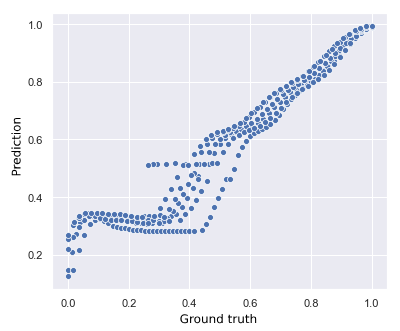
\includegraphics[scale=0.48,width=\textwidth]{figures/traj-without-stop-compression3.png}
    \caption{Estimated trajectory progression for new data without stop compression.}
    \label{fig:progression-without-stop-compression}
  \end{minipage}
  \hspace{5pt}
  \begin{minipage}{.46\textwidth}
    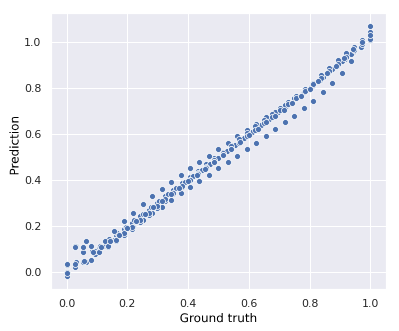
\includegraphics[scale=0.5,width=\textwidth]{figures/traj-with-stop-compression3.png}
    \caption{Estimated trajectory progression for new data with stop compression.}
    \label{fig:progression-with-stop-compression}
  \end{minipage}
\end{figure}

\noindent
This assumption did not hold with data points clustered on the same spot, so to make the assumption work, all the data points generated during a stand-still were clustered into one with the mean values of all clustered points. Without this compression, the trajectory used to learn $f^{(r,s)}_s$ also mattered a lot, since where it stopped during a journey would greatly affect the estimated synchronisation function. As shown in figures~\ref{fig:progression-without-stop-compression} and~\ref{fig:progression-without-stop-compression}, the estimated progression much more closely resemble the actual progression when stop compression is used, indicated by the linear relationship.

\subsubsection{Support Data}
In addition to requiring the data to be uniformly distributed, it was essential that $f^{(r,s)}_s$ was a smooth mapping with respect to the direction of spatial progress. That is, data points close in spatial progression should be mapped onto points in $\tau$ which are also close. Furthermore, data distributed orthogonally to the direction of spatial progression should be mapped onto the same point in $\tau$. This requirement is quite reasonable when one considers that a bus driving slightly more to the left on a road is no closer to its destination than a bus driving slightly more to the right. Another motivation for this is that the GPS data includes some measurement error which has to be considered in the synchronisation.

\begin{figure}[H]
  \begin{minipage}{.46\textwidth}
    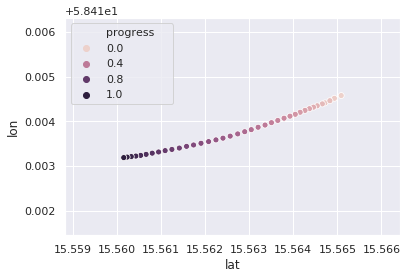
\includegraphics[scale=0.48,width=\textwidth]{figures/traj-without-support-data2.png}
    \caption{Spatial progression of trajectory~2.}
    \label{fig:traj-without-support-data}
  \end{minipage}
  \hspace{5pt}
  \begin{minipage}{.46\textwidth}
    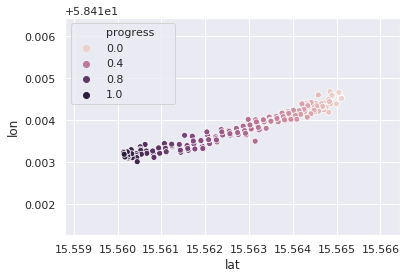
\includegraphics[scale=0.5,width=\textwidth]{figures/traj-with-support-data2.png}
    \caption{Spatial progression of support data~2.}
    \label{fig:traj-with-support-data}
  \end{minipage}
\end{figure}

\noindent
In order to force the GP to model a function with this property, each data point $d^{(i)}$ was duplicated by placing a normal distribution over it, orthogonal to the spatial progression vector ${(d^{(i+1)}_x - d^{(i)}_x, d^{(i+1)}_y - d^{(i)}_y)}^T$, and drawing several samples with the same progression as $d^{(i)}$. This process is illustrated in figures~\ref{fig:traj-without-support-data} and~\ref{fig:traj-with-support-data}. The generated support data was saved to a separate data set and combined with the trajectory data when training synchronisation GPs.

\begin{figure}[H]
  \begin{minipage}{.46\textwidth}
    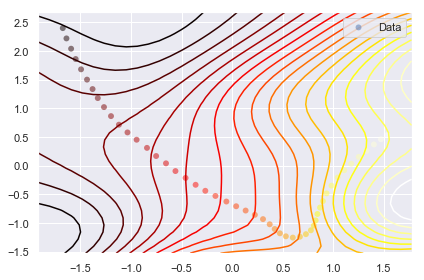
\includegraphics[scale=0.48,width=\textwidth]{figures/heat-without-support-data.png}
    \caption{Heightmap of a synchronisation GP without using support data.}
    \label{fig:heightmap-without-support}
  \end{minipage}
  \hspace{5pt}
  \begin{minipage}{.46\textwidth}
    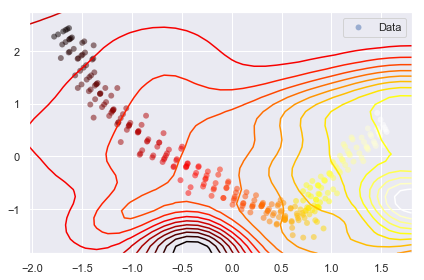
\includegraphics[scale=0.5,width=\textwidth]{figures/heat-with-support-data.png}
    \caption{Heightmap of a synchronisation GP using support data.}
    \label{fig:heightmap-with-support}
  \end{minipage}
\end{figure}

\noindent
As shown in figures~\ref{fig:heightmap-without-support} and~\ref{fig:heightmap-with-support}, using support data greatly increase how orthogonal the contours of $f^{(r,s)}_s$ are to the spatial progression, which indicate the desired properties.

\subsection{Prediction}
After the synchronisation GPs was trained, it was possible to train the model for making the actual predictions. Training was done by first mapping all the training trajectories onto $\tau$ using the set of learned  $f^{(r,s)}_s$, and then training two GPs to the synchronised trajectory. The first one was the inverse of the synchronisation GP, ${GP_s^{(t, r,s)}}^{-1}$, which modeled ${f^{(t, r,s)}_s}^{-1}(\tau) : \tau \mapsto \mathcal{R}^2$, and the second was the actual prediction GP $GP_p^{(t,r,s)}$, which modeled ${f^{(t,r,s)}_p}^{-1}(\tau) : \tau \mapsto \mathcal{R}$, which predicted arrival time as a scalar from synchronised progression. Both of these were stored to disk, to be loaded as needed when presented with a new trajectory on the corresponding segment $(r, s)$.

The purpose of ${GP_s^{(t,r,s)}}^{-1}$ was to acquire log likelihoods for new data $(\bar{x}, \bar{y})$, which was given by
\begin{equation}
  \label{eq:model-log-likelihood}
  \begin{split}
    \log P(\bar{y}|\bar{x}, {GP_s^{(t, r,s)}}^{-1}) & = -\frac{1}{2}(\bar{y} - \mu(\bar{x}){[\Sigma]}^{-1}(\bar{x} - \mu(\bar{y}) \\
    & = -\frac{1}{2}\log{|\Sigma|}+C,
  \end{split}
\end{equation}
where $\mu(\bar{x})$ and $\Sigma(\bar{x})$ are given by equations~\ref{eq:gp-mean-function}, and~\ref{eq:gp-covariance-function} for a specific ${GP_s^{(t, r,s)}}^{-1}$. Since ${GP_s^{(t,r,s)}}^{-1}$ and $GP_p^{(t,r,s)}$ were trained on the same $t$, it was true that $\log P(\bar{y}|\bar{x}, GP_p^{(t, r,s)})$ was also given by equation~\ref{eq:model-log-likelihood}, which with Bayes theorem gave the unnormalised log distribution
\begin{equation}
  \label{eq:model-log-model-probability}
  \log P(GP_p^{(t, r,s)} | \bar{y}, \bar{x}) \propto \log P(\bar{y}|\bar{x}, GP_p^{(t, r,s)}) + \log P(GP_p^{(t, r,s)})
\end{equation}
over models, where a uniform prior was assumed. The prediction for a model was then given by
\begin{equation}
  \label{eq:model-prediction-probability}
  P(\bar{y}|\bar{x}, GP_p^{(t, r,s)}) \propto P(\bar{y}|\bar{x}, GP_p^{(t, r,s)})P(GP_p^{(t, r,s)} | \bar{y}, \bar{x})
\end{equation}
where Bayes theorem was once again used.
\begin{figure}[H]
    \caption{Density comparison}
  \begin{subfigure}[b]{0.5\textwidth}
    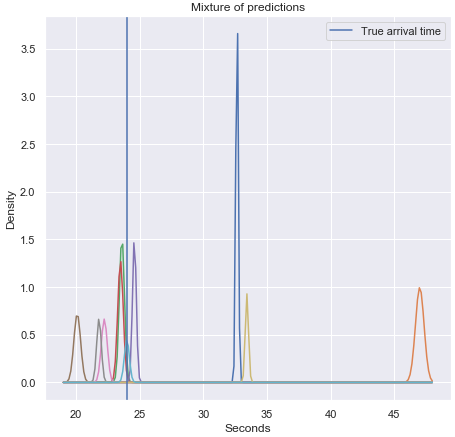
\includegraphics[width=\textwidth]{figures/mixture-start-of-traj.png}
    \caption{Density of arrival times at the start of a segment.}
    \label{fig:mixture-start-of-traj}
  \end{subfigure}
  %
  \begin{subfigure}[b]{0.5\textwidth}
    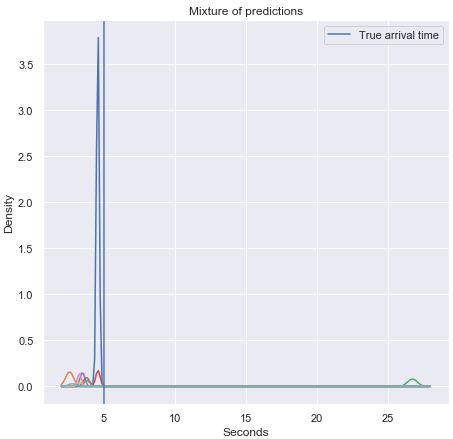
\includegraphics[width=\textwidth]{figures/mixture-end-of-traj.png}
    \caption{Density of arrival times at the end of a segment.}
    \label{fig:mixture-end-of-traj}
  \end{subfigure}
\end{figure}
\noindent
The distribution over arrival times $P(\bar{y} | \bar{x})$ was finally given by a mixture of predictions
\begin{equation}
  \label{eq:model-mixture}
  P(\bar{y} | \bar{x}) = \sum_{t}{\pi_{t}P(\bar{y}|\bar{x}, GP_p^{(t, r,s)})}
\end{equation}
for all models previously learned, where the mixture weights $\pi_k$ was given by $P(GP_p^{(t, r,s)} | \bar{y}, \bar{x})$ according to equation~\ref{eq:model-prediction-probability}. The model made predictions by taking the mean of this distribution. Figure~\ref{fig:mixture-start-of-traj} and figure~\ref{fig:mixture-end-of-traj} show how the models certainty increases as a trajectory progresses, which is because  a larger part of the trajectory is revealed, which improves the weightings in the mixture distribution.

%%%%%%%%%%%%%%%%%%%%%%%%%%%%%%%%%%%%%%%%%%%%%%%%%%%%%%%%%%%%%%%%%%%%%%
%%% lorem.tex ends here

%%% Local Variables: 
%%% mode: latex
%%% TeX-master: "demothesis"
%%% End: 
